\chapter{The importance of parameter values in the clustering output}

\section{Monocle and Seurat}
As stated in the previous chapter, the PhenoGraph pipeline was widely adopted in the task of processing biological data, due to its efficiency and quality of results. The pipeline was incorporated and implemented in various programming languages.

The most frequently used R packages that perform single-cell data processing are Seurat (currently on the third version) \cite{Hao2021} and Monocle (currently at the third version) \cite{Cao2019}. Both packages use the PhenoGraph method for the cell clustering. The goal of this chapter is to evaluate the output of the two packages and compare the results side by side.

\section{Data used for experiments}
To perform this comparison, we used the Cuomo data \cite{Cuomo2020}, an in-vitro SMART-seq dataset of human endoderm differentiation. The dataset contains 1880 cells extracted from six donors (hayt, naah, vils, pahc, melw and qunz) at four different timepoints. The cells are in expressed in approximately 30 000 genes. The dataset was preprocessed by removing the cells that are expressed in less than 200 features and the genes that are expressed in less than three cells. MT (mitochondrial) and RP (ribosomal protein) genes were also excluded from the feature set.

The purpose of this thesis is to analyze the clustering pipeline, therefore the preprocessing parameters (normalization and scaling) are done in the same manner for both packages.

\section{Algorithms used in the pipeline}
In chapter one we presented the steps that are involved in the PhenoGraph pipeline, namely the dimensionality reduction, the graph construction and the community detection. Each step can be performed by a varying number of algorithms. Therefore, in order to compare the two R packages, we must identify the algorithms that they are using in the clustering pipeline (see Table \ref{tab:s4-m3-methods}).

For the dimensionality reduction, both packages allow the usage of either linear methods (PCA) or non-linear ones (UMAP and tSNE). The developers of the both packages recommend performing the PCA reduction on the raw data, followed by tSNE or UMAP. The graph construction is performed using the kNN based method. For the community detection, Monocle uses the Louvain and Leiden alogrithms, whereas Seurat can cluster the cells using Louvain with multi-level refinement and SLM, too.


\begin{table}[]
    \begin{tabular}{|l|l|l|l|}
        \hline
                               & \textbf{Dim reduction}    & \textbf{Graph construction} & \textbf{Graph clustering}                                                                                                                                                                                                                                                                                                                                                              \\ \hline
        \textbf{Seurat}        & \begin{tabular}[c]{@{}l@{}}PCA followed\\ by tSNE or UMAP\end{tabular} & \begin{tabular}[c]{@{}l@{}}kNN based\\ support for SNN\end{tabular}   & \begin{tabular}[c]{@{}l@{}}Louvain, Louvain refined,\\ SLM, Leiden\end{tabular}                                                                                                                                                                                                                                                                                                                                                              \\ \hline
        \textbf{Monocle}       & \begin{tabular}[c]{@{}l@{}}PCA followed\\ by tSNE or UMAP\end{tabular} & \begin{tabular}[c]{@{}l@{}}kNN based\\ support for SNN\end{tabular}   & Louvain, Leiden                                                                                                                                                                                                                                                                                                                                                                        \\ \hline
        \textbf{Used packages} & \begin{tabular}[c]{@{}l@{}}PCA: \verb|irlba| \tablefootnote{GitHub official repository: \url{https://github.com/bwlewis/irlba}}\\ tSNE: \verb|Rtsne| \tablefootnote{GitHub official repository: \url{https://github.com/jkrijthe/Rtsne}} \\ UMAP: \verb|uwot| \tablefootnote{GitHub official repository: \url{https://github.com/jlmelville/uwot}}\end{tabular} & \begin{tabular}[c]{@{}l@{}}kNN: \verb|RANN| \tablefootnote{GitHub official repository: \url{https://github.com/jefferislab/RANN}} \end{tabular}   & \begin{tabular}[c]{@{}l@{}}Louvain: \verb|igraph| \tablefootnote{GitHub official repository: \url{https://github.com/igraph/igraph}}\\        Leiden: \verb|leidenbase| \tablefootnote{GitHub official repository: \url{https://github.com/cole-trapnell-lab/leidenbase}} , \\\verb|leiden| \tablefootnote{GitHub official repository: \url{https://github.com/TomKellyGenetics/leiden}}\end{tabular}  \\ \hline
    \end{tabular}
    \caption{\label{tab:s4-m3-methods}The algorithms used by Monocle and Seurat inside the Phenograph pipeline}
\end{table}

\section{Comparing the results}

\begin{figure}[H]
    \centering
    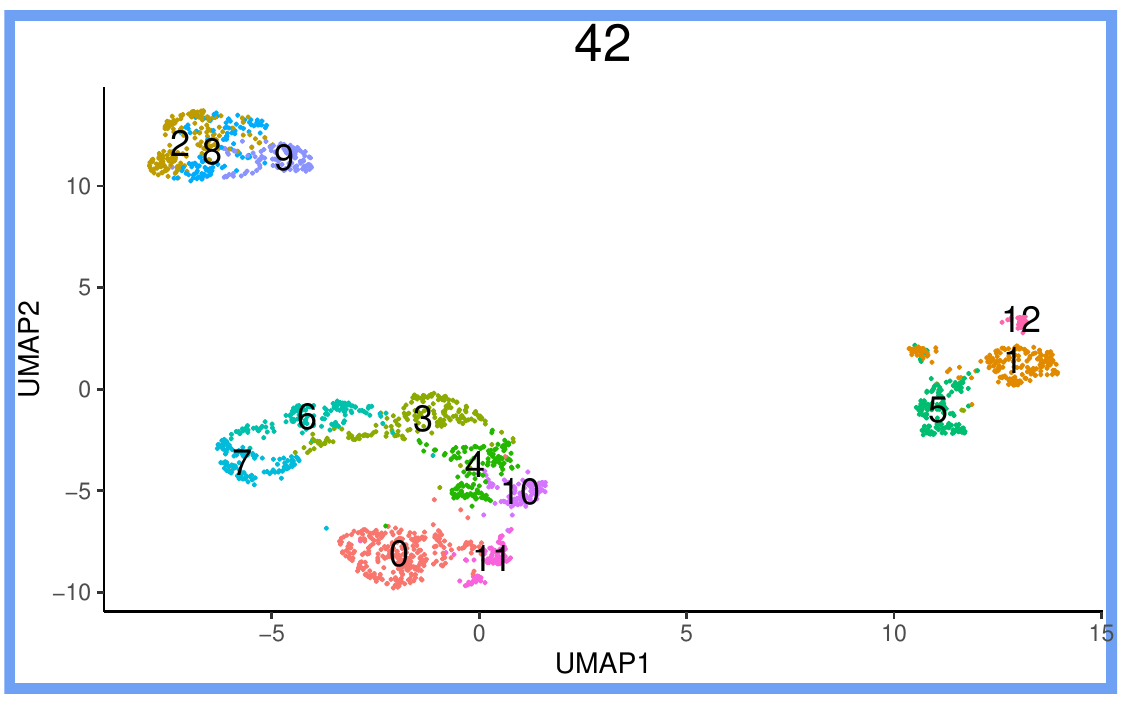
\includegraphics[width=7cm]{ch2/2_S1.png}
    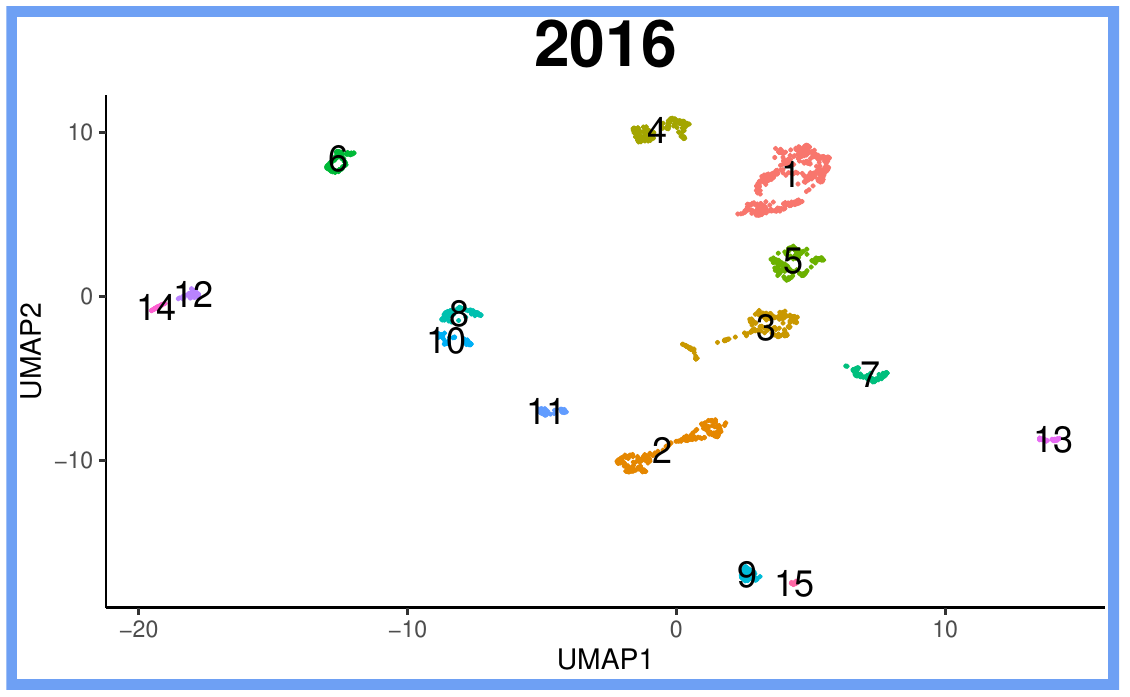
\includegraphics[width=7cm]{ch2/2_M1.png}
    \caption{\label{fig:s4-m3-default}Clustering distribution with default parameters for Monocle (right) and Seurat (left). The title indicates the default random seed that is used.}
\end{figure}

If the Cuomo \cite{Cuomo2020} dataset is clustered using the Monocle and Seurat packages with default parameters, significantly different outputs are produced, as it can be observed in Figure \ref{fig:s4-m3-default}. Firstly, there are differences with respect to the dimensionality reduction. The cells are scattered in multiple islands in the Monocle package, whereas Seurat obtains a more compact grouping. Also, the two packages disagree regarding the number of clusters: Seurat outputs 13 clusters, Monocle 15.

The biological interpretation of the data heavily relies on the clusters' structure. Thus, is expected for the discrepancies between the two packages to extend over the marker identification and the biological interpretation. The question we pose is whether the divergence between Monocle and Seurat has technical (such as the implementation of the clustering pipeline) or biological (such as additional pre- or post-processing steps that rely on the sequencing information) causes.

\section{Aligning the results}
We started by analyzing the tehnical differences between the two packages. This involves implementation discrepancies, but also different values of the parameters involved in the clustering process. Our analysis will follow the PhenoGraph pipeline and we will compare the two packages regarding the three steps.

\subsection{Seed}
All algorithms involved in the clustering pipeline contain at least one stochastic component, therefore it is expected that using different random seeds might impact the clustering result. By default, Monocle uses 2016 as random seed, and Seurat 42. Figure \ref{fig:s4-m3-seed} shows how changing the seed affects the topology: in some cases, the changes are equivalent to some rotations of the groups, but there can be noticable differences inside a group's structure (as it can be observed for the island in the right side of the two panels).

\begin{figure}[H]
    \centering
    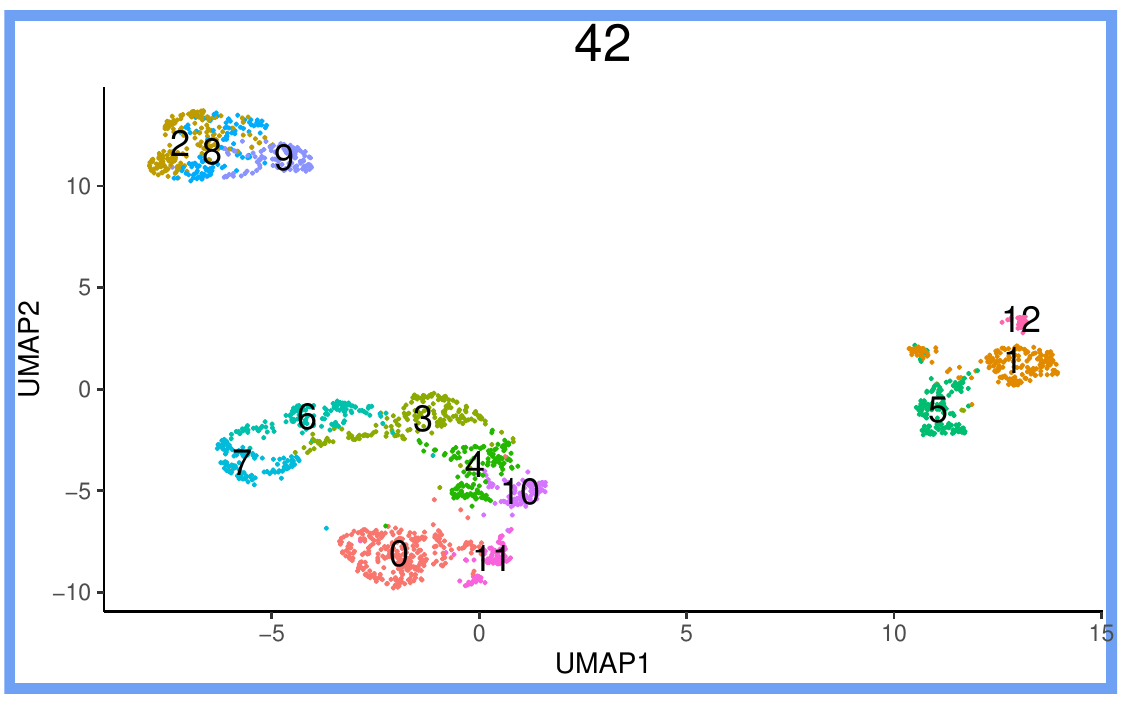
\includegraphics[width=7cm]{ch2/2_S1.png}
    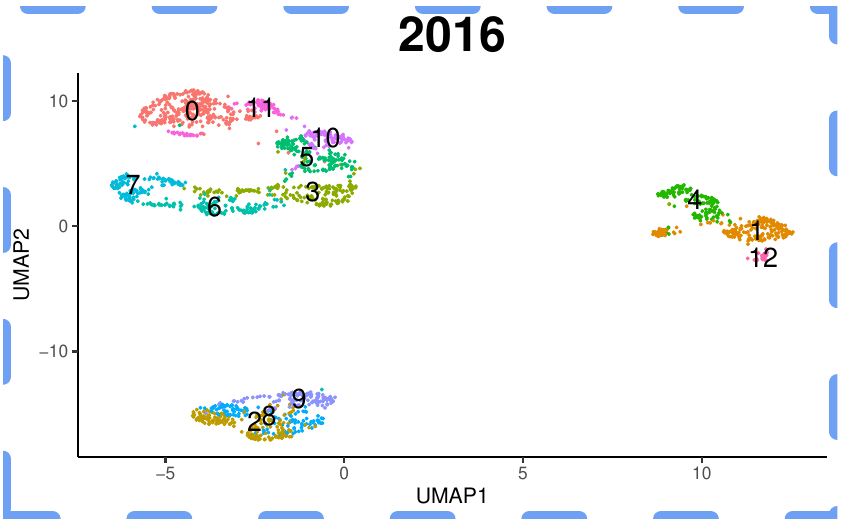
\includegraphics[width=7cm]{ch2/2_S2.png}
    \caption{\label{fig:s4-m3-seed}Clustering distribution with default parameters for Monocle (right) and Seurat (left). The title indicates the default random seed that is used.}
\end{figure}.

\subsection{Dimensionality reduction}
As stated in the previous sections, both Seurat and Monocle suggest applying PCA on the raw dataset and UMAP or tSNE afterwards. The default choice for non-linear dimensionality reduction is UMAP. As for the implementation, both packages are using the same R packages: \verb|irlba| for PCA (citation) and \verb|uwot| for UMAP (citaton).

\subsubsection{PCA}
The output of the PCA can be affected by parameters such as the number of principal components or the precision of the calculation (the \verb|irlba| package performs an approximate PCA calculation), but the difference between the packages lies in the feature space. Although the data contains up to 30 000 genes, most of them are not appropiate for describing the cells behaviour, as they would introduce more noise than perform any significant separation. Thus, the standard in the processing of the biological data is to choose a relatively small subset of genes that contain discriminative information. By default, Monocle uses all genes, but Seurat performs the PCA only on the genes that have the most variability (citation) (also reffered in literature as highly variable - or HV - genes). Figure \ref{fig:s4-m3-pca} illustrates how the feature set affects the topology. If Seurat uses all genes for PCA, the resulting embedding will contain numerous small islands (see panels S3 and S4). Using only HV genes in Monocle leads to more compact group of cells (see panels M3 and M4).

\subsubsection{UMAP}
The UMAP algorithm is signifcantly affected by three parameters:
\begin{itemize}
    \item \textit{the distance metric} that is used in the original space
    \item \textit{the number of neighbours} that is used for building the graph
    \item \textit{the minimum distance} which determines how separated should points be in the low dimensional space. Low values lead to dense groups, while higher values are more preferable for visualisation.
\end{itemize}

Monocle and Seurat agree on the cosine measurement as the distance metric, but the other two parameters have different values in these packages: the minimum distance is 0.3 in Seurat and 0.1 in Monocle, and the number of neighbours is 30 in Seurat and 15 in Monocle. Figures \ref{fig:s4-m3-min-dist} and \ref{fig:s4-m3-n-neigh-umap} highlight the effect of these parameters on the toplogy of the data. Aligning their values for the two packages leads to identical low dimensional representation of the cells, as it can be seen in panels S7 and M8 of the figure \ref{fig:s4-m3-n-neigh-umap}.

\begin{figure}[H]
    \centering
    \makebox[\textwidth][c]{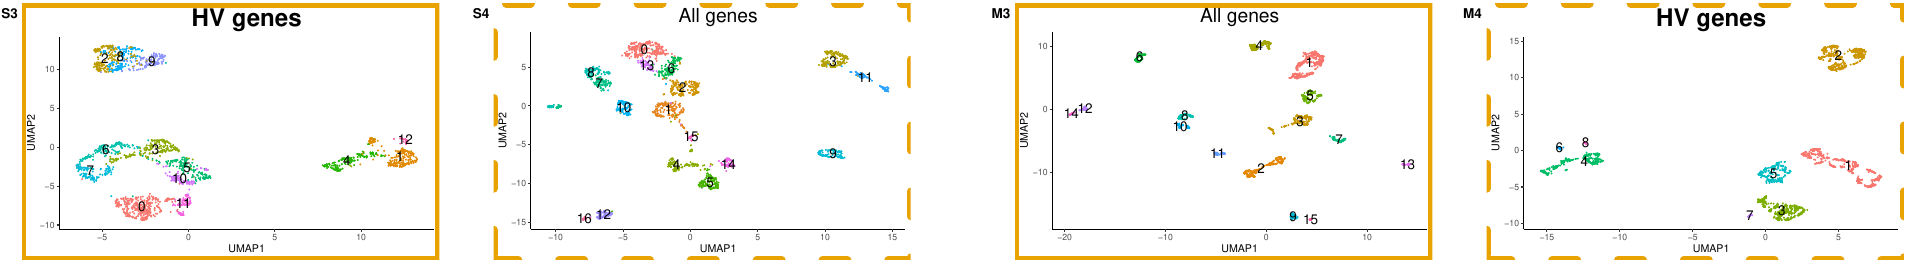
\includegraphics[width=1.2\linewidth]{ch2/2_pca_genes.png}}
    \caption{\label{fig:s4-m3-pca}Clustering distribution with default parameters for Monocle (left) and Seurat (right). The title indicates the default random seed that is used.}
\end{figure}


\begin{figure}[H]
    \centering
    \makebox[\textwidth][c]{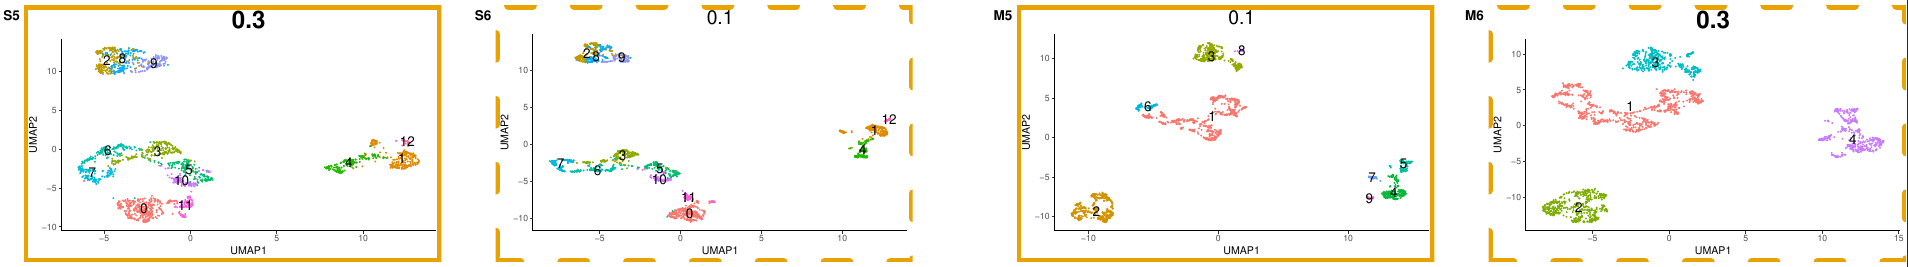
\includegraphics[width=1.2\linewidth]{ch2/2_umap_min_dist.png}}
    \caption{\label{fig:s4-m3-min-dist}Clustering distribution with default parameters for Monocle (left) and Seurat (right). The title indicates the default random seed that is used.}
\end{figure}

\begin{figure}[H]
    \centering
    \makebox[\textwidth][c]{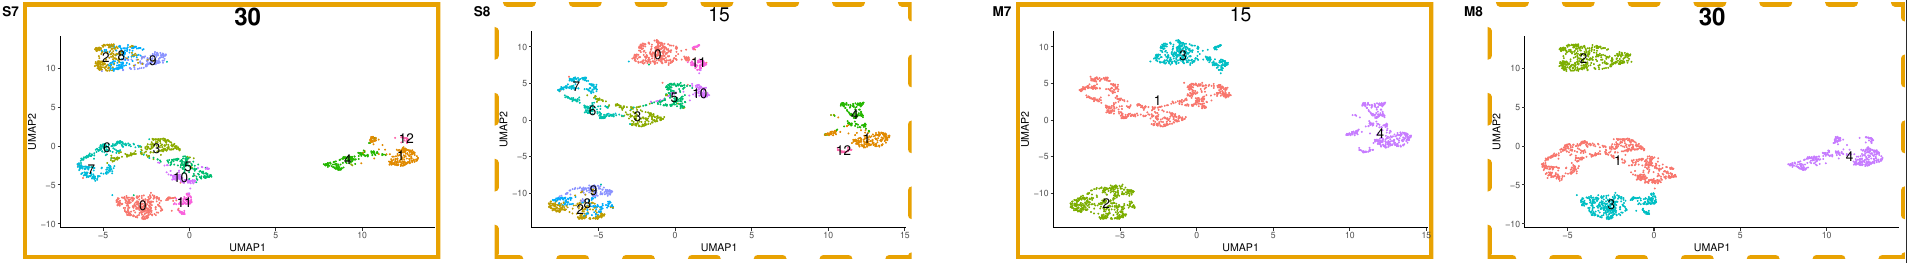
\includegraphics[width=1.2\linewidth]{ch2/2_umap_n_neigh.png}}
    \caption{\label{fig:s4-m3-n-neigh-umap}Clustering distribution with default parameters for Monocle (left) and Seurat (right). The title indicates the default random seed that is used.}
\end{figure}

\subsection{Graph construction}
Both packages use the kNN-based method of building the graph based on the reduced space. The calculation of the nearest neighbours is done by the method implemented in the \verb|RANN| package. The output is affected by the embedding that is used as a base for the graph construction, the number of neighbours (or simply \textit{k}) and the graph type.

Both Monocle and Seurat agree upon the value of 20 nearest neighbours. As for the base embedding, Seurat builds the graph on the reduced space obtained by PCA, while Monocle uses the low dimensional data from UMAP. As Figure \ref{fig:s4-m3-graph-base} suggests, changing the base embedding can affect the clustering output. On the Cuomo data, the number of clusters is lower when PCA is used as base embedding compared to UMAP for both packages (this can be observed by comparing panels S9 with S10 an M9 with M10 respectively).

When it comes to calculating the Shared Nearest Neighbour graph, the two packages have their own implementation. Although they are synonymous in the most of the cases, there are some differences that impact the final structure of the resulting graph.

\subsubsection{Self-neighbours}
The major discrepancy between them relates to the usage of the self-neighbours. A \textit{self-neighbour} refers to label a point as a near neighbour of itself. Seurat uses self-neighbours, while Monocle doesn't.

The importance of self-neighbours is illustrated on Figure \ref{fig:s4-m3-snn-1}. Setting $k = 5$, we calculate the neighbourhoods for the fourth and the fifth points. If we include the self-neighbour, we get:

\[ \begin{aligned}
        N_5(4) = \{4,5,3,1,2\} & \\
        N_5(5) = \{5,4,3,2,1\}
    \end{aligned}
\]

Given that the SNN graph is calculated using the Jaccard Similarity Index of the neighbourhoods, the weight of the edge between these two nodes will be:

\[ W_{4,5} = \textrm{JSI}(N_5(4), N_5(5)) = \frac{|N_5(4) \cap N_5(5)|}{|N_5(4) \cup N_5(5)|} = \frac{5}{5} = 1 ,\]

which indicates a perfect similarity between the two points. However, not including the self-neighbours leads to the following results:

\[ \begin{aligned}
        N_5(4) = \{5,3,1,2,6\} & \\
        N_5(5) = \{4,3,2,1,7\}
    \end{aligned}
\]

The intersection between these neighbourhoods contains only three points, and the union contains seven. Thus, the weight assigned in this case would be $3 / 7 = 0.43$. Even if we decrease the value of $k$ from 5 to 4, the JSI would be $3 / 5 = 0.6$, which still does not reflect or indicate the reality of a perfect similarity between the two nodes.

Another discrepancy is presented in the example provided in the Figure \ref{fig:s4-m3-snn-2}. Using the same value for $k$, we calculate the neighbourhoods for the first and the sixth point. If we include the self-neighbour, we get:

\[ \begin{aligned}
        N_5(1) & = \{1,2,3,4,6\} \\
        N_5(6) & = \{6,7,8,9,1\}
    \end{aligned}
\]

The neighbourhoods sets of these two points point out that they are direct neighbours. Therefore, the weight of the edge between them is expected to be non-zero: $\displaystyle \frac{|N_6(4)  \cap N_6(6)|}{|N_6(4)  \cup N_6(6)|} = \frac{2}{8} = 0.25$. Excluding the self-neighbours leads to disjoint neighbourhoods:

\[ \begin{aligned}
        N_5(1) & = \{2,3,4,6,5\}  \\
        N_5(6) & = \{7,8,9,1,10\}
    \end{aligned}
\]

Thus, not using the self-neighbours leads to the false conclusion that there is no similarity between direct neighbours.

\subsubsection{Indirect neighbours}
Another implementation difference between Seurat and Monocle relates to the indirect neighbour. We consider two points to be \textit{indirect neighbours} if the intersection of their neighbourhoods is not disjoint. Looking at the third and eighth points from the example from Figure \ref{fig:s4-m3-snn-1} when $k = 6$, the intersection between their neighbourhoods is not empty ($\{5, 7\}$ for Seurat and $\{5,7,4,6\}$ for Monocle).

Even if the intersection is not empty, Monocle discards any use of the indirect neighbours. Thus, there will be an edge between two nodes only if they are direct neighbours.

\subsubsection{Scaling the weights}
Following the conclusion of the previous two differences, we can state that Monocle cannot build a graph that has an edge with weight 1.

\begin{proof} From the first difference, Monocle does not include the self-neighbours, therefore points that are direct neighbours will always have the JSI less than one, as the intersection will not include the points themselves. The only way to reach a perfect similarity is to have two points that are not direct neighbours, but share the same neighbourhood.

    However, from the second difference, we know that in Monocle indirect neighbours are not taken into consideration. Therefore, even if we would obtain an edge with a weight of one between the two points, it will be discarded, given the restriction.
\end{proof}

The developers of the Monocle package decided to solve this limitation by performing a scaling of the weights to the interval $[0, 1]$. The issue of this approach is that it can affect the clustering output and the downstream partitioning result, as some quality function are scale variant (citation).

\subsubsection{Case study}
To prove the importance of these differences between the two implementations, we used the Cuomo \cite{Cuomo2020} dataset. The number of nearest neighbours is set to $k = 150$. Figure \ref{fig:s4-m3-snn-3} illustrates the difference between Monocle and Seurat results, shown for the neighbours of a point chosen from the datset.

The first two panels present the weight distribution of the edges incident to the chosen point when using Seurat (A) and Monocle (B). The third panel contains the absolute difference of the weights of the edges incident to direct neighbours. As it can be observed, the maximum difference is not greater than 0.012, which suggests that the two implementations behave similarly for direct neighbours when $k$ is reasonably high. Panel D shows the distribution of the weights incident to the indirect neighbours. The colour scale indicates that there is a reasonable amount of points where the weight has a value that may have an impact in the overall structure of the final graph.

\subsubsection{Aligning the SNN implementations}
After the analysis of the two implementations of the algorithm of building the SNN graph, we concluded that Seurat's is a more suitable choice.

However, continuing the alignment process between the two packages, the graph type parameters is different. Seurat is building the SNN (the weighted) graph, while Monocle builds the unweighted one. The impact of this parameter is presented in the Figure \ref{fig:s4-m3-n-graph-type}, which suggests that using a weighted version of the same graph is influencing the clustering output.

\begin{figure}[H]
    \centering
    \makebox[\textwidth][c]{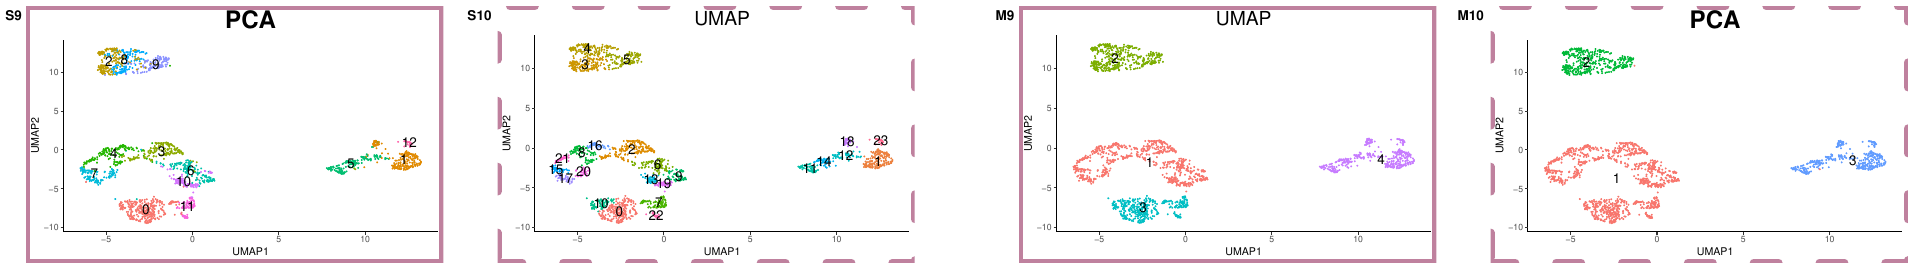
\includegraphics[width=1.2\linewidth]{ch2/2_graph_base.png}}
    \caption{\label{fig:s4-m3-graph-base}Clustering distribution with default parameters for Monocle (left) and Seurat (right). The title indicates the default random seed that is used.}
\end{figure}

\begin{figure}[H]
    \centering
    \makebox[\textwidth][c]{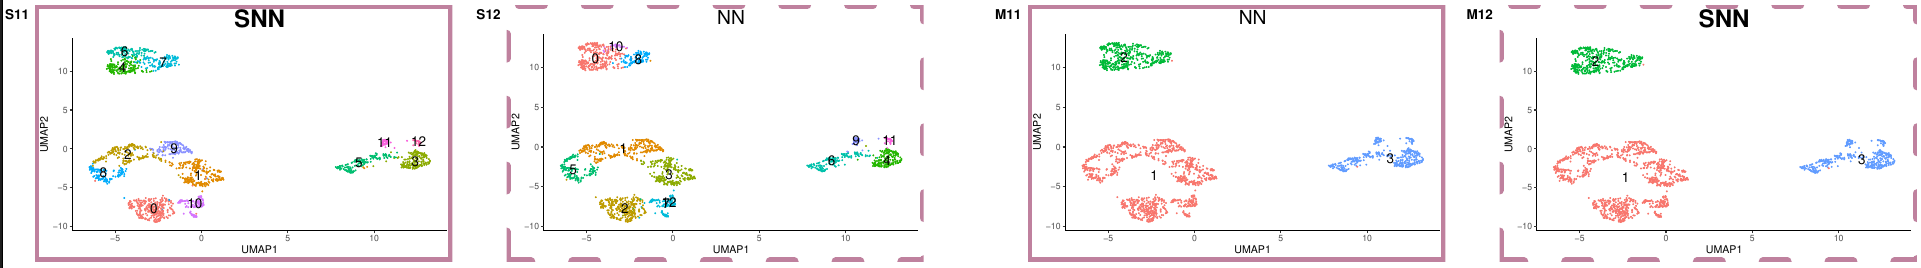
\includegraphics[width=1.2\linewidth]{ch2/2_graph_type.png}}
    \caption{\label{fig:s4-m3-n-graph-type}Clustering distribution with default parameters for Monocle (left) and Seurat (right). The title indicates the default random seed that is used.}
\end{figure}

\begin{figure}[H]
    \centering
    \makebox[\textwidth][c]{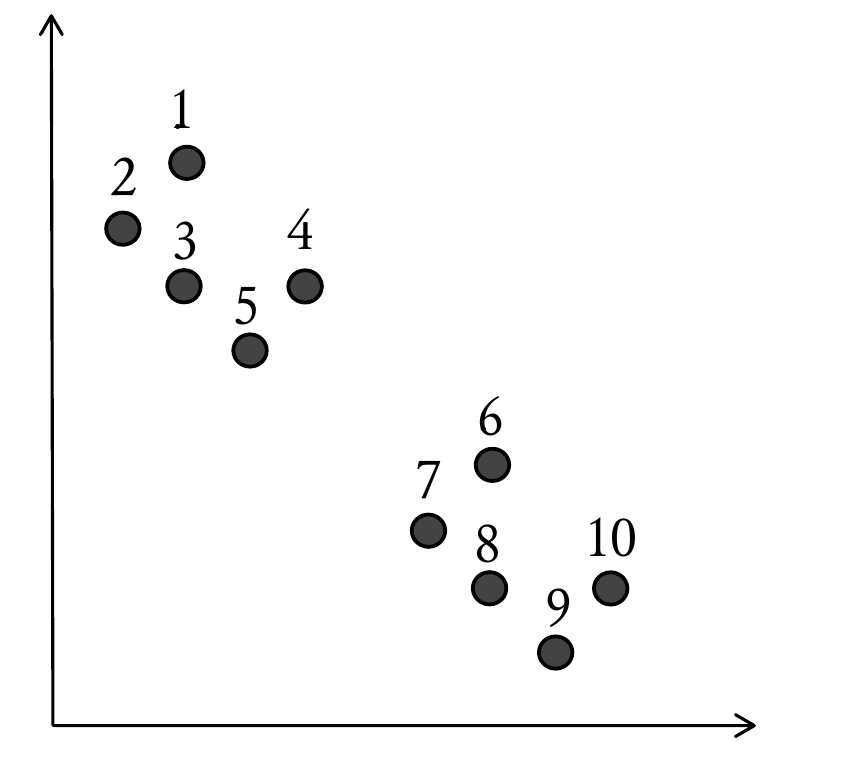
\includegraphics[width=5cm]{ch2/2_snn_issue_1.png}}
    \caption{\label{fig:s4-m3-snn-1}Clustering distribution with default parameters for Monocle (left) and Seurat (right). The title indicates the default random seed that is used.}
\end{figure}

\begin{figure}[H]
    \centering
    \makebox[\textwidth][c]{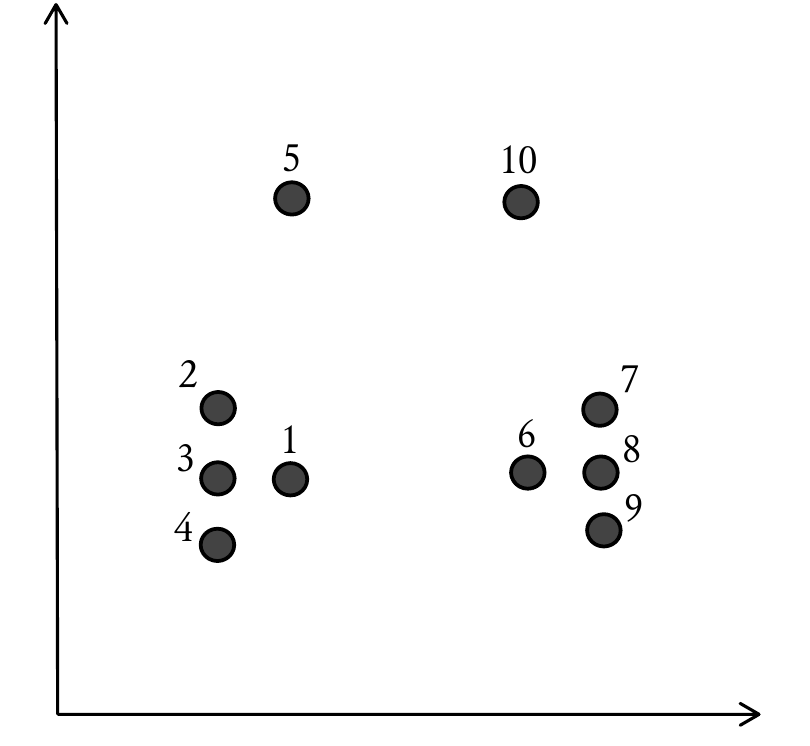
\includegraphics[width=5cm]{ch2/2_snn_issue_2.png}}
    \caption{\label{fig:s4-m3-snn-2}Clustering distribution with default parameters for Monocle (left) and Seurat (right). The title indicates the default random seed that is used.}
\end{figure}

\begin{figure}[H]
    \centering
    \makebox[\textwidth][c]{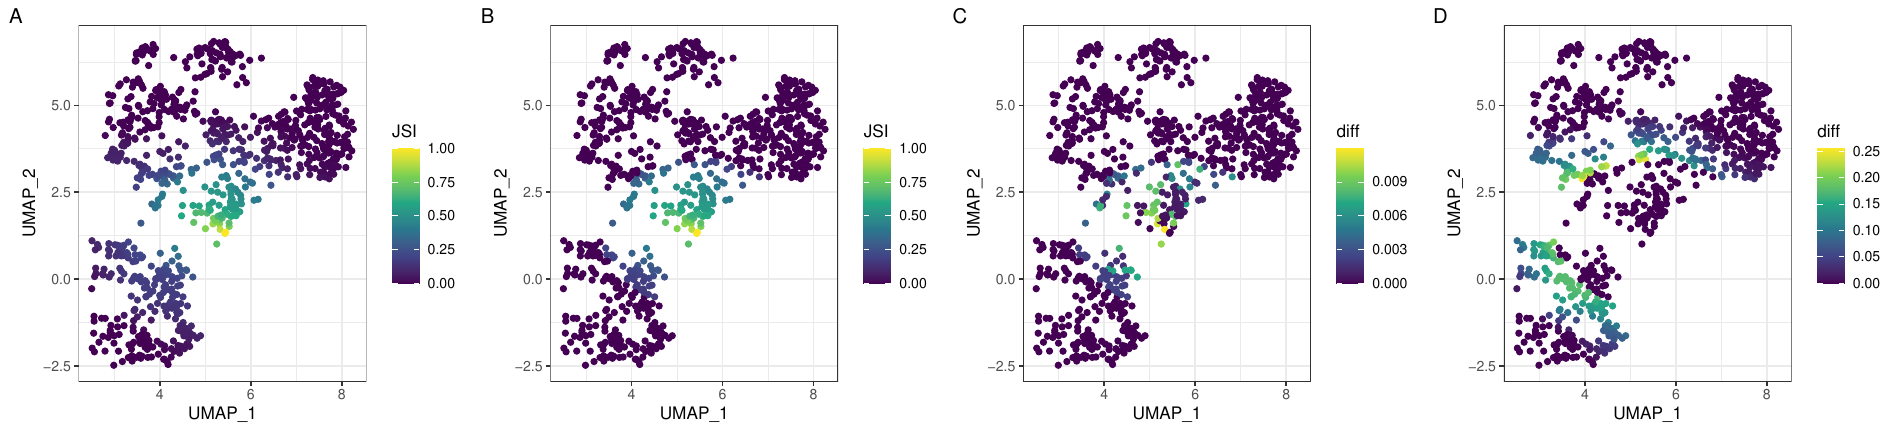
\includegraphics[width=1.2\textwidth]{ch2/2_snn_issue_3.png}}
    \caption{\label{fig:s4-m3-snn-3}Clustering distribution with default parameters for Monocle (left) and Seurat (right). The title indicates the default random seed that is used.}
\end{figure}

\subsection{Graph clustering}
Once the two packages reach an agreement on the low-dimensional reduced space and on the built graph, the clustering step must be aligned in order to obtain the same partitions. Firstly, both Seurat and Monocle should use the same clustering alogrithms. By default, Monocle clusters data using the Leiden algorithm and Seurat uses the Louvain algorithm. In Figure \ref{fig:s4-m3-graph-alg} we can observe how the two community detection methods produce a different output on the same graph.

Given the optimization nature of the clustering algorithm, the objective function is another important parameter that can influence the composition of the clusters, as it can be seen in \ref{fig:s4-m3-quality}. It is noticeable how the CPM quality function, used by default by Monocle, leads to getting more clusters compared to the RBConfiguration function which is used by Seurat.

The parameter that directly influences the number of clusters is the resolution parameter. Monocle sets the resolution to $1e-4$ and Seurat to $0.8$. Figure \ref{fig:s4-m3-res} proves the intuition that using different resolution values outputs different number of clusters.

Finally, the community detection algorithms are iterative, thus using a different number of iterations might lead to different results, especially in the cases where no convergence is reached. Monocle uses by default a number of 2 iterations, while Seurat 10. The difference between the clusterings can be seen in the left panel of Figure \ref{fig:s4-m3-cont}, which is a contingency table between the partitions obtained by the two package. To get a perfect match between the two, the matrix should be diagonal, but in our case there are three cases of non-zero entries outside the diagonal.

\begin{figure}[H]
    \centering
    \makebox[\textwidth][c]{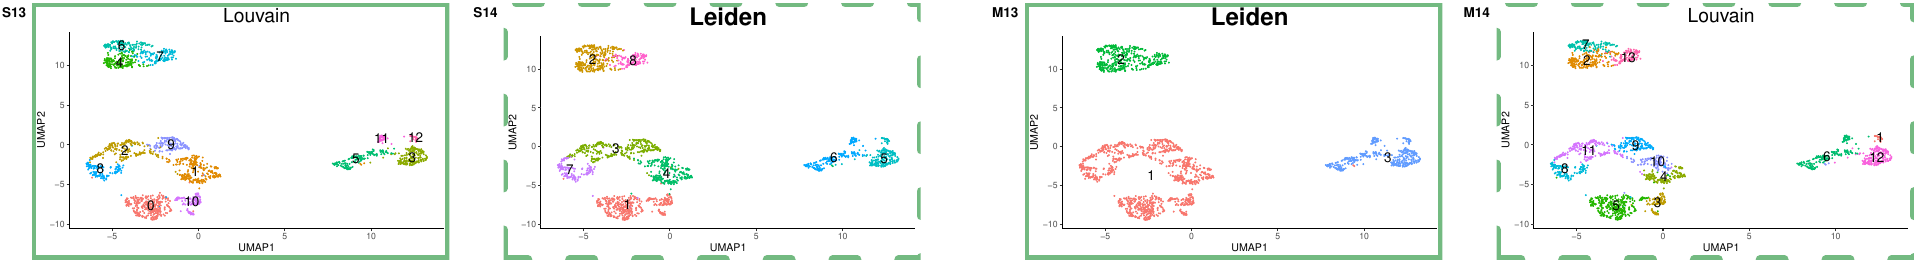
\includegraphics[width=1.2\linewidth]{ch2/2_graph_alg.png}}
    \caption{\label{fig:s4-m3-graph-alg}Clustering distribution with default parameters for Monocle (left) and Seurat (right). The title indicates the default random seed that is used.}
\end{figure}

\begin{figure}[H]
    \centering
    \makebox[\textwidth][c]{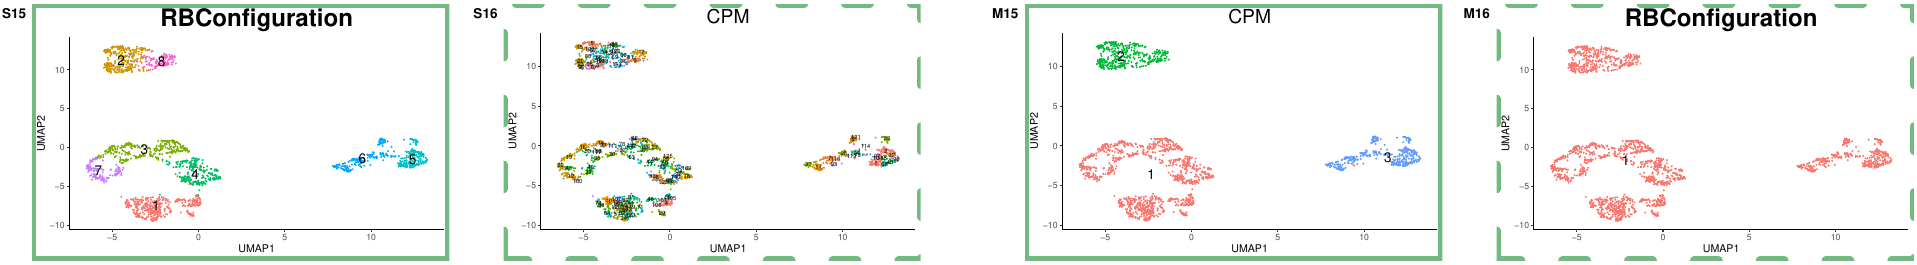
\includegraphics[width=1.2\linewidth]{ch2/2_quality_function.png}}
    \caption{\label{fig:s4-m3-quality}Clustering distribution with default parameters for Monocle (left) and Seurat (right). The title indicates the default random seed that is used.}
\end{figure}

\begin{figure}[H]
    \centering
    \makebox[\textwidth][c]{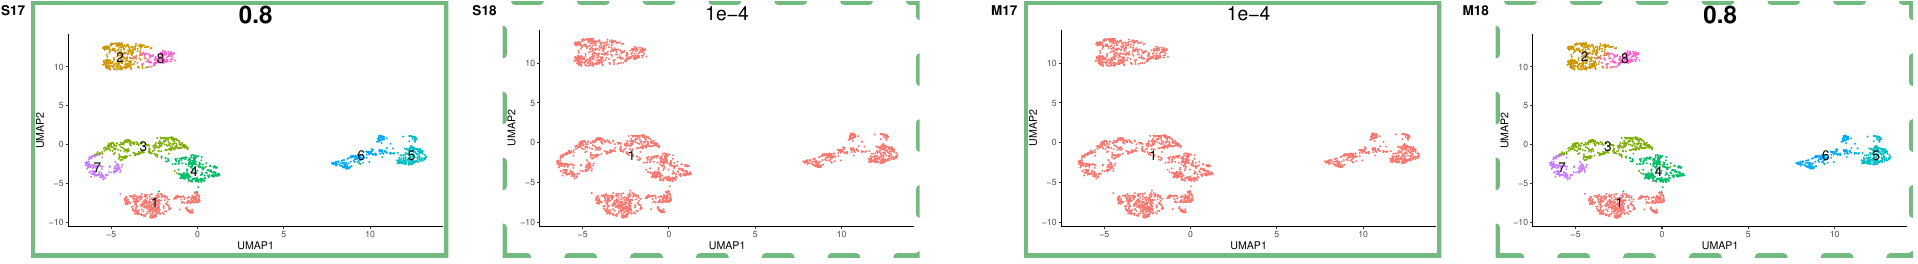
\includegraphics[width=1.2\linewidth]{ch2/2_resolution.png}}
    \caption{\label{fig:s4-m3-res}Clustering distribution with default parameters for Monocle (left) and Seurat (right). The title indicates the default random seed that is used.}
\end{figure}


\begin{figure}[H]
    \centering
    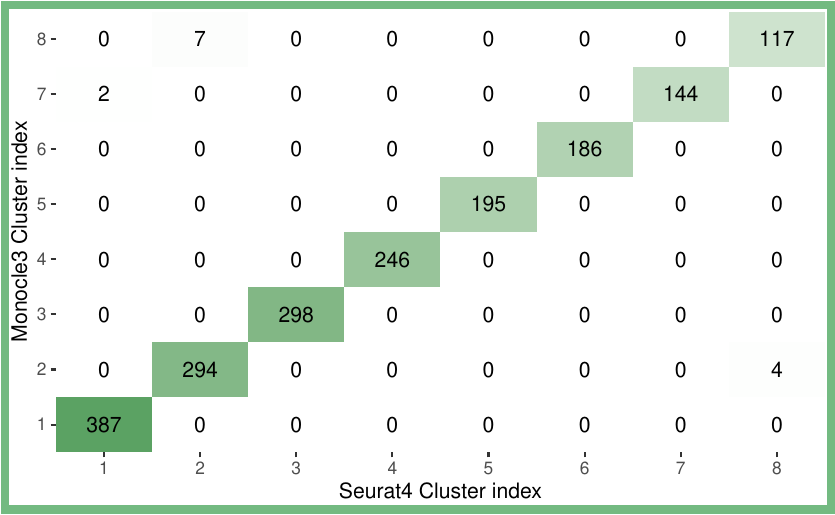
\includegraphics[width=0.3\linewidth]{ch2/2_cont_table.png}
    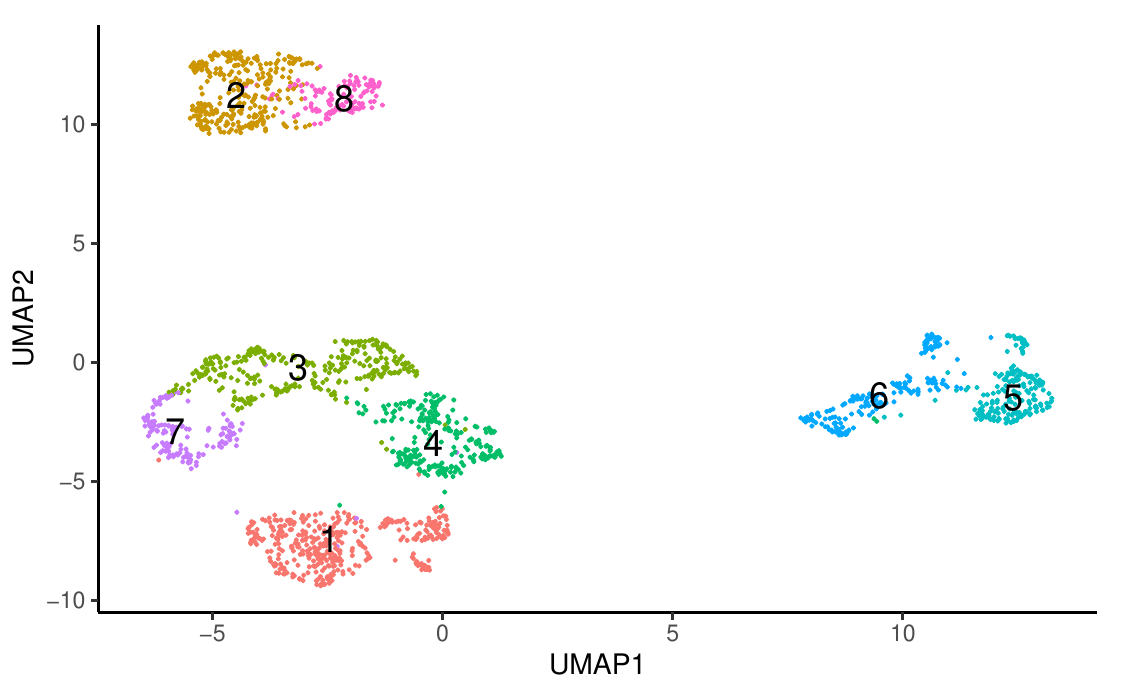
\includegraphics[width=0.3\linewidth]{ch2/2_final_clustering.png}
    \caption{\label{fig:s4-m3-cont}Clustering distribution with default parameters for Monocle (left) and Seurat (right). The title indicates the default random seed that is used.}
\end{figure}

\section{Summary}
After performing all the aligning steps (summarized in Table \ref{tab:param}), both packages obtain the same partition (shown in the right display of Figure \ref{fig:s4-m3-cont}).

The conclusion is that the initial differences between Seurat and Monocle were caused by technical factors, namely different implementation of the method or different values for the important parameters.

% Please add the following required packages to your document preamble:
% \usepackage[table,xcdraw]{xcolor}
% If you use beamer only pass "xcolor=table" option, i.e. \documentclass[xcolor=table]{beamer}
\begin{table}[]
    \resizebox{\textwidth}{!}{
        \begin{tabular}{|l|l|l|l|}
            \hline
            \textbf{Parameter name}     & \textbf{Step}                            & \textbf{Monocle value}     & \textbf{Seurat value}      \\ \hline
            \textbf{seed}               & \cellcolor[HTML]{6D9FF3}-                & 2016                       & 42                         \\ \hline
            \textbf{feature set}        & \cellcolor[HTML]{E7A101}Dim reduction    & all genes                  & HV genes                   \\ \hline
            \textbf{UMAP min dist}      & \cellcolor[HTML]{E7A101}Dim reduction    & 0.1                        & 0.3                        \\ \hline
            \textbf{UMAP n neighbours}  & \cellcolor[HTML]{E7A101}Dim reduction    & 15                         & 30                         \\ \hline
            \textbf{base embedding}     & \cellcolor[HTML]{BE809D}Graph building   & UMAP                       & PCA                        \\ \hline
            \textbf{SNN implementation} & \cellcolor[HTML]{BE809D}Graph building   & \begin{tabular}[c]{@{}l@{}}no self-neighbours\\ only direct neighbours\end{tabular} & \begin{tabular}[c]{@{}l@{}}with self-neighbours\\ direct and indirect neighbours\end{tabular} \\ \hline
            \textbf{graph type}         & \cellcolor[HTML]{BE809D}Graph building   & unweighted                 & weighted                   \\ \hline
            \textbf{clustering method}  & \cellcolor[HTML]{72B980}Graph clustering & Leiden                     & Louvain                    \\ \hline
            \textbf{quality function}   & \cellcolor[HTML]{72B980}Graph clustering & CPM                        & RBConfiguration            \\ \hline
            \textbf{resolution}         & \cellcolor[HTML]{72B980}Graph clustering & 1e-4                       & 0.8                        \\ \hline
            \textbf{\#iterations}       & \cellcolor[HTML]{72B980}Graph clustering & 2                          & 10                         \\ \hline
        \end{tabular}}
    \caption{\label{tab:param}The parameters that affect the output of the clustering pipeline.}
\end{table}